\section{Resultados}

\begin{frame}
\centering
\huge
Resultados de tiempo 
    
\end{frame}

\begin{frame}{Tiempos de inferencia}

\framesubtitle{DIGITS}
	\begin{columns}
		\column{.1\textwidth}
 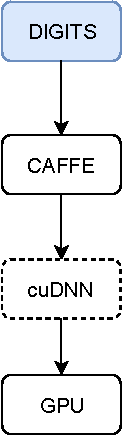
\includegraphics[width=1\textwidth]{diagrama/frame1.pdf}
        
        \column{.85\textwidth}
	\begin{figure}[H]
	\centering
 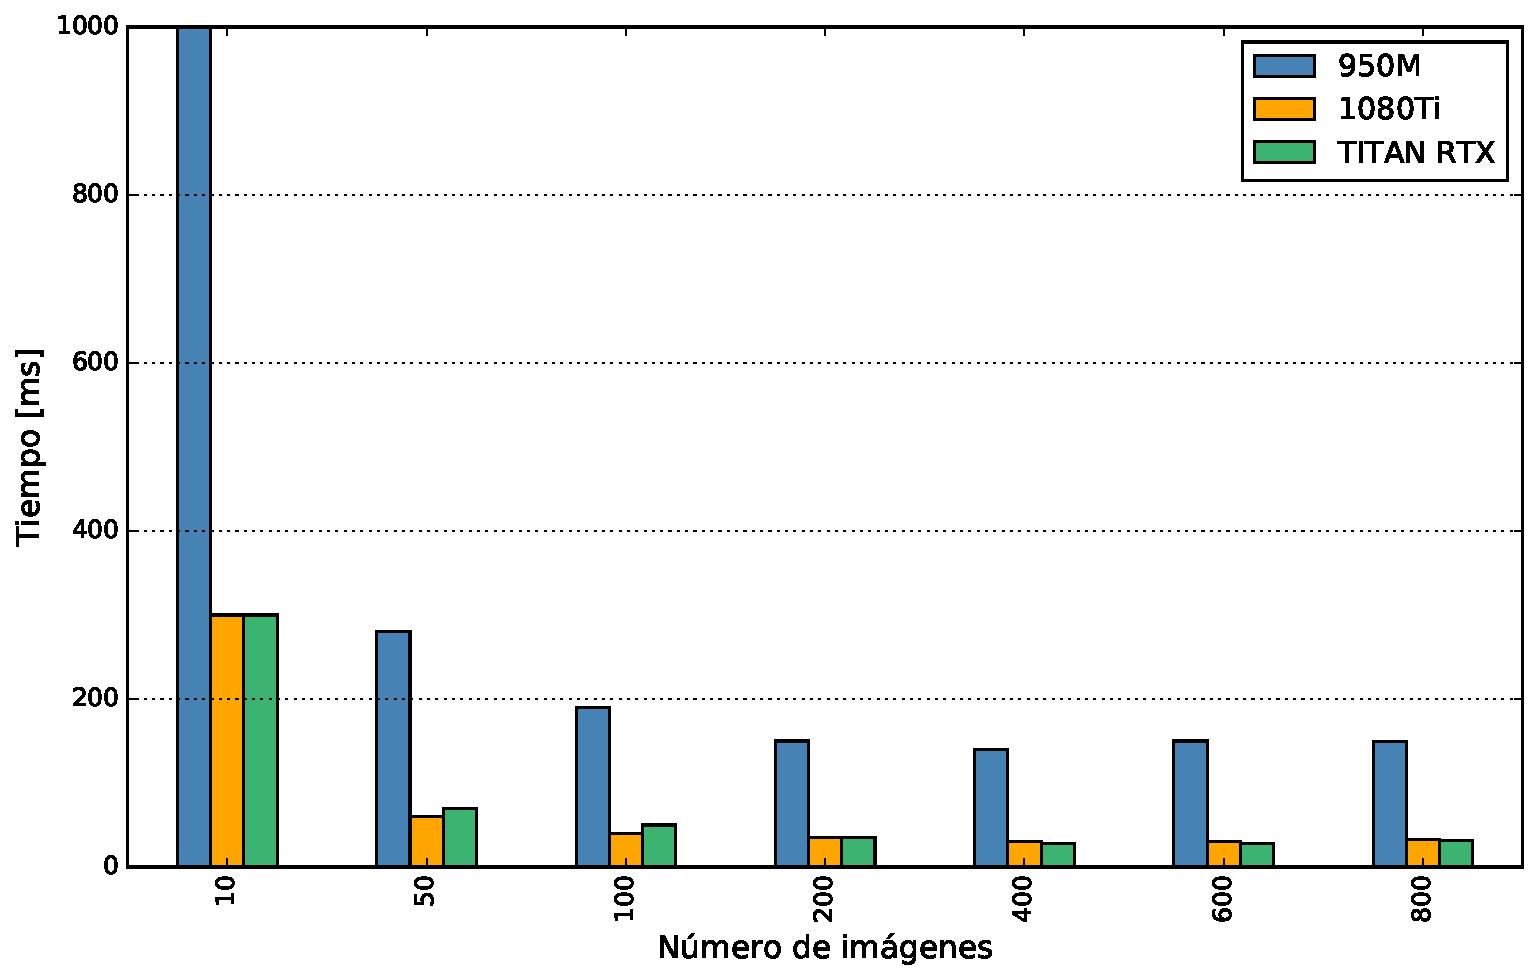
\includegraphics[width=1\textwidth]{barplot/digits.pdf}
	\end{figure}
	\end{columns}
 
\end{frame}



\begin{frame}{Tiempos de inferencia}

\framesubtitle{Caffe}
	\begin{columns}
		\column{.1\textwidth}
 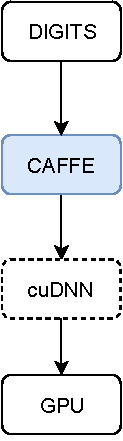
\includegraphics[width=1\textwidth]{diagrama/frame2.pdf}
        
        \column{.85\textwidth}
	\begin{figure}[H]
	\centering
 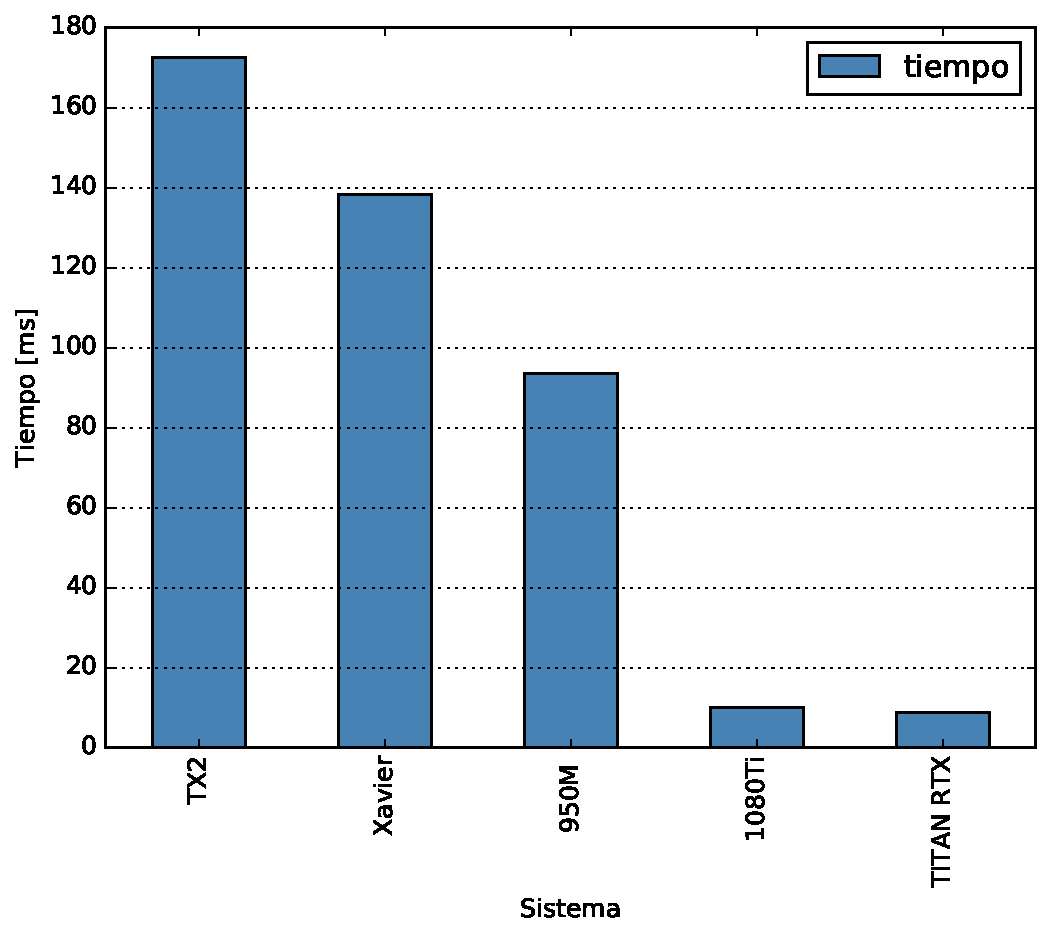
\includegraphics[width=0.7\textwidth]{barplot/avg-fire.pdf}
	\end{figure}
	\end{columns}
 
\end{frame}





\begin{frame}{Tiempos por capa}
\framesubtitle{FCN AlexNet}
	\centering
 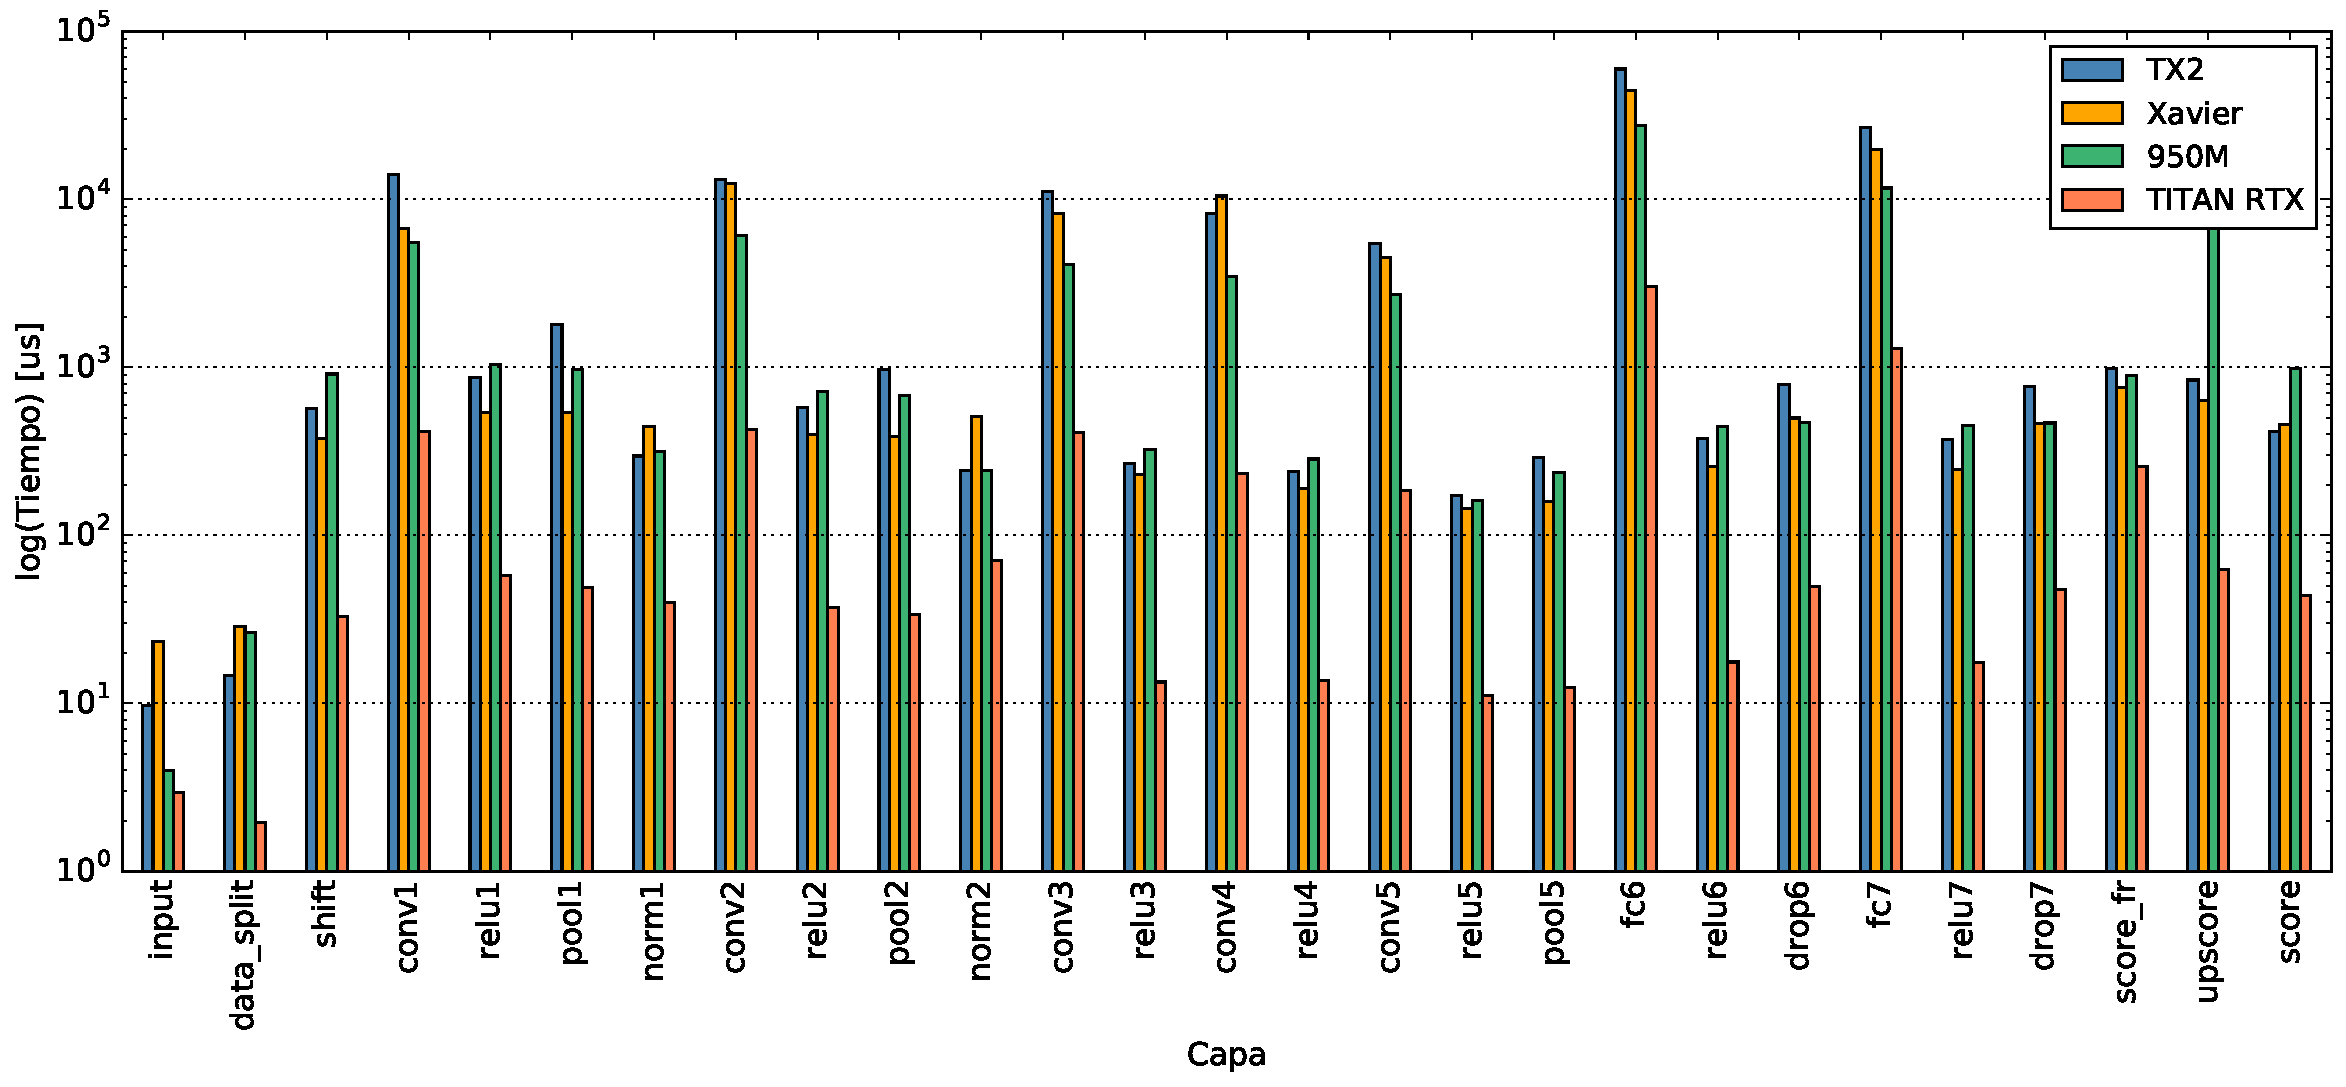
\includegraphics[width=1\textwidth]{barplot/layers-alex.pdf}

\end{frame}

\begin{frame}{Tiempos por capa}
\framesubtitle{Simple Feature Extraction}
	\centering
 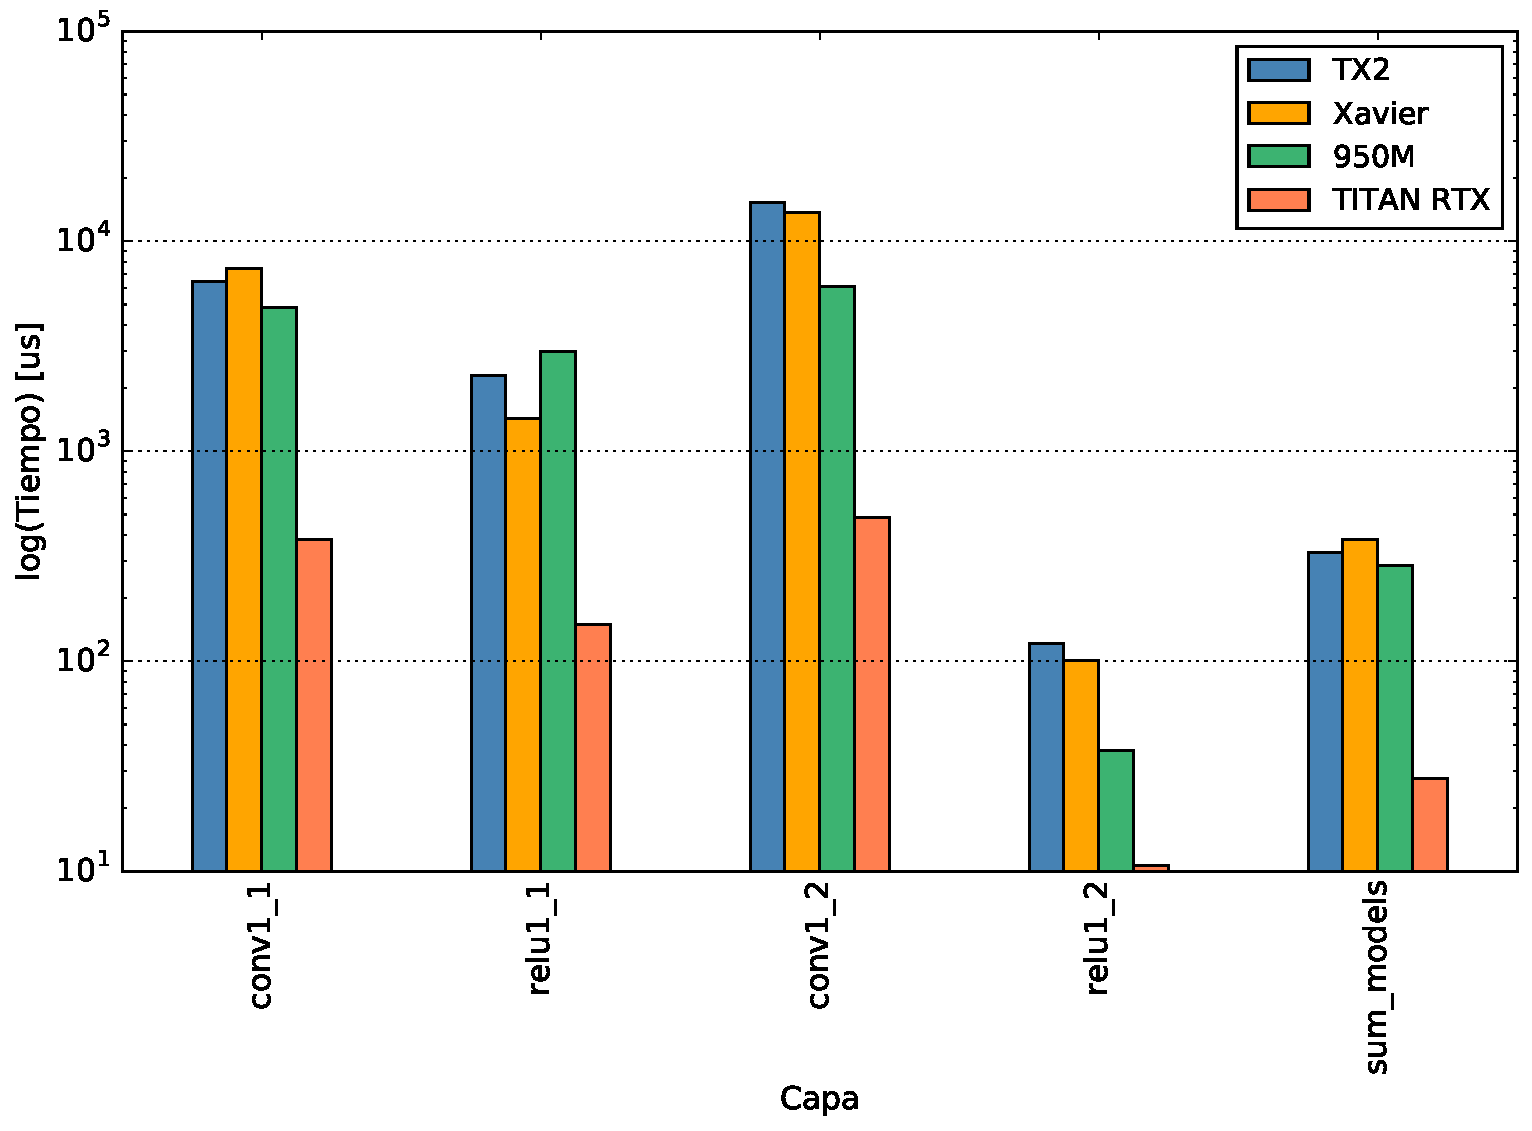
\includegraphics[width=0.7\textwidth]{barplot/layers-sfe.pdf}

\end{frame}



 
\begin{frame}{Tiempos por función}
\framesubtitle{Análisis de dependencias Jetson TX2}
\centering
\resizebox{0.75\linewidth}{!}{


\begin{table}[]
\centering

\begin{tabular}{lcc}
\toprule
Kernel   & Critical path {[}\%{]} & Critical path {[}s{]} \\
\midrule
cuDNN GEMM      & 43.84                  & 39.56                  \\
cuDNN ReLU      & 7.47                   & 6.75                   \\
CPU other & 5.5                    & 4.96                   \\
cuDNN Winograd  & 2.73                   & 2.46       \\
\bottomrule
\end{tabular}

\end{table}
}
\end{frame}


\begin{frame}{Tiempos por función}
\framesubtitle{Análisis de dependencias Jetson AGX Xavier}
\centering
\resizebox{0.75\linewidth}{!}{
\begin{table}[]
\centering

\begin{tabular}{lcc}
\toprule
Kernel      & \multicolumn{1}{l}{Critical path {[}\%{]}} & \multicolumn{1}{l}{Critical path {[}s{]}} \\
\midrule
cuDNN GEMM         & 58.65                                      & 5.47                                      \\
Caffe im2col & 7.7                                        & 0.74                                      \\
CPU other    & 5.84                                       & 0.56                                      \\
Caffe ReLU   & 0.84                                       & 0.08    \\
\bottomrule
\end{tabular}

\end{table}
}
\end{frame}



\begin{frame}{Tiempos por llamada API CUDA}
	\begin{columns}
		\column{.1\textwidth}
 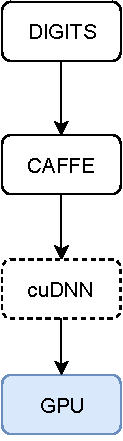
\includegraphics[width=1\textwidth]{diagrama/frame4.pdf}
        
        \column{.85\textwidth}
	\begin{figure}[H]
	\centering
 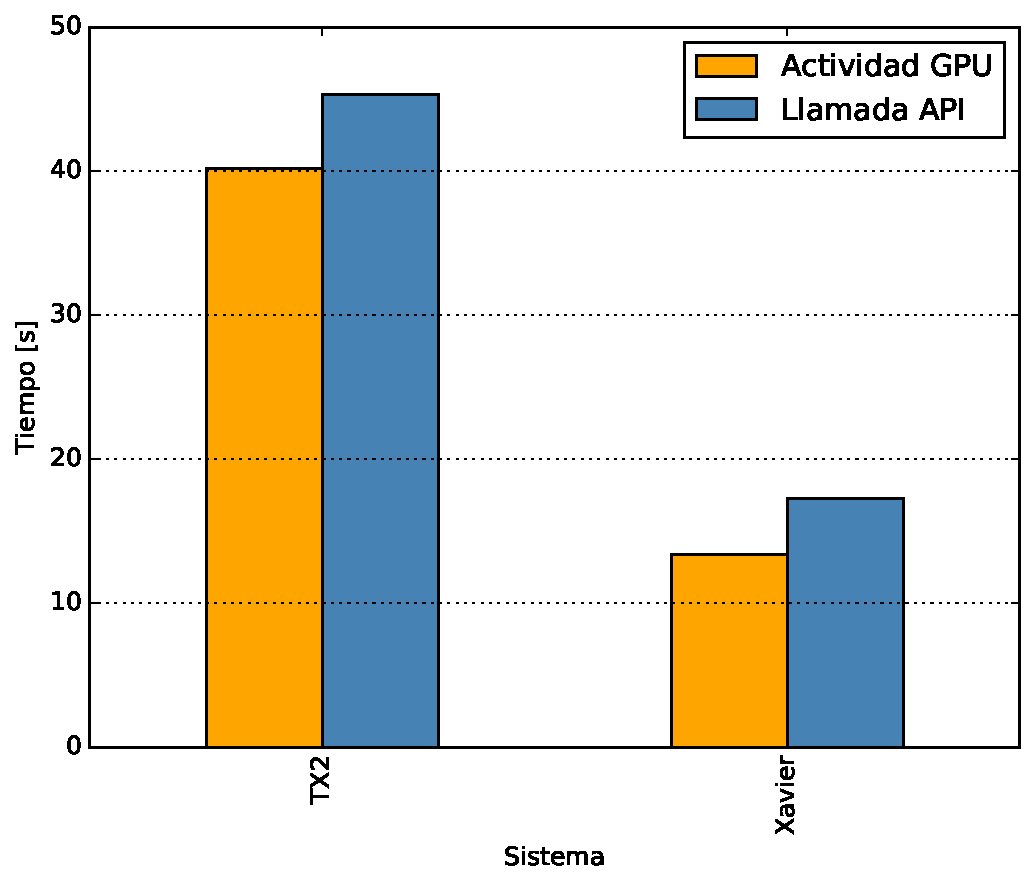
\includegraphics[width=0.7\textwidth]{barplot/gpu-act.pdf}
	\end{figure}
	\end{columns}
\end{frame}
 
\begin{frame}{Tiempos por llamada de API CUDA}
\framesubtitle{Análisis de dependencias Jetson TX2}
\resizebox{\linewidth}{!}{


\begin{table}[]
\centering

\begin{tabular}{lccccc}
\toprule
Llamada API              & Critical path {[}\%{]} & Critical path {[}s{]} & Tiempo espera {[}s{]} \\
\midrule
Stream create with flags & 28.14                  & 25.41                 & 0.00                  \\
cuda Free                 & 1.82                   & 1.64                  & 0.00                  \\
cuda Event Synchronize        & 0.64                   & 0.58                  & 58.58                \\
\bottomrule
\end{tabular}

\end{table}
}
\end{frame}


\begin{frame}{Tiempos por llamada de API CUDA}
\framesubtitle{Análisis de dependencias Jetson AGX Xavier}
\resizebox{\linewidth}{!}{
\begin{table}[]
\centering

\begin{tabular}{lccc}
\toprule
Llamada API   & Critical path {[}\%{]} & Critical path {[}s{]} & Tiempo espera {[}s{]} \\
\midrule
cuda Free      & 15.91                  & 1.53                  & 0.00                  \\
cuda Malloc    & 0.66                   & 0.63                  & 0.00                  \\
cuda Event Synchronize & 0.42                   & 0.04                  & 3.35                 \\
\bottomrule
\end{tabular}

\end{table}
}
\end{frame}


